\section{An Example}
\label{sec-example}

% Intro
To illustrate the key benefits of \toolname\, we show an example in
Figure~\ref{fig-git}. Figure~\ref{fig-git} visually represents the update protocol for two
commands of Git, a popular source-code version control software~\cite{git}. It
is widely used for collaborative software development like the Linux kernel. 

We first describe the update protocol diagram (\sref{sec-protocol-diagram}),
explain the protocol (\sref{sec-protocol-explain}), and then describe the
vulnerabilities that were found by \toolname (\sref{sec-git-vul}). We then show
how \toolname\ can relate the vulnerabilities back to application source code
(\sref{sec-git-patch}).  

\subsection{Git Protocol Diagram}
\label{sec-protocol-diagram}
\begin{figure}[!t]
\centering
\vspace{-0.2in}
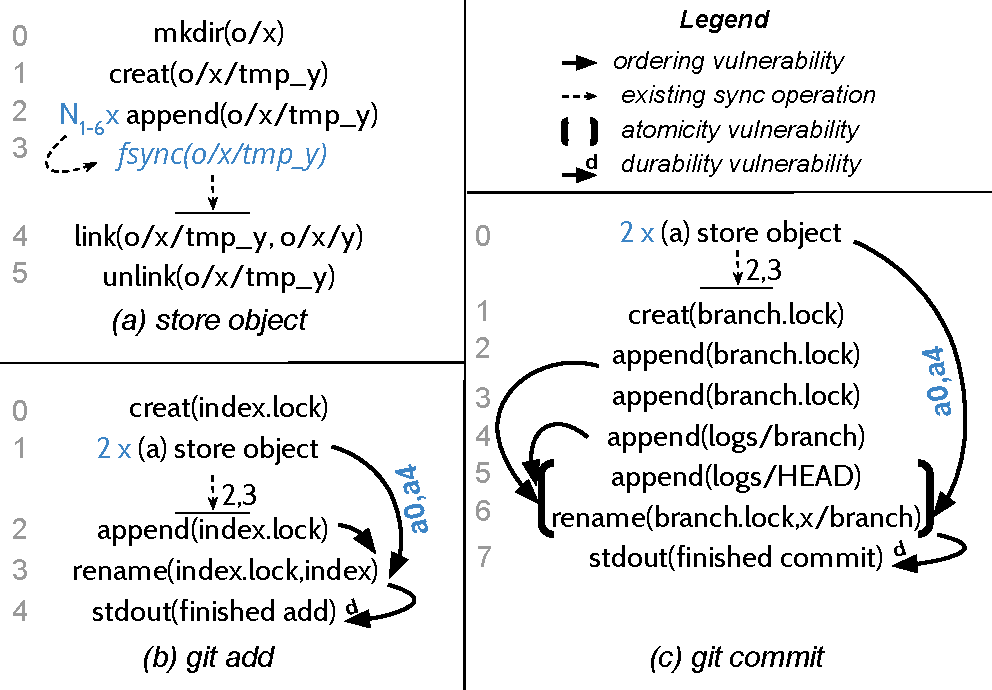
\includegraphics[scale=0.47]{figs/git2.pdf}
\vspace{-0.1in}
\mycaption{fig-git}{Git Update Protocol}{\footnotesize The figure shows the
update protocol of Git broken up into modules. The dark arrows and brackets represent
new dependencies discovered by \toolname. The dashed arrows represent
known dependencies. Numbers on the arrow represent the lines of
the source module that need to be persisted before the destination. We observe that
even though Git is a mature, well-tested application, crash vulnerabilities
exist in common tasks such as add and commit.
}
\vspace{-0.2in}
\end{figure}




Protocol diagrams help understand the update protocol by preserving the core
logic while hiding distracting low-level details. The protocol diagram
represents \textit{logical operations} in the update protocol, rather than
system calls. Operations are organized together as modules. Questions such as
what are the main techniques used (e.g., atomic rename, write-ahead-logging,
etc.) can be answered easily. All the ordering and atomicity vulnerabilities
are shown clearly -- file-system developers may be able to use this to figure
out if the application can run consistently on their file system. Without
\toolname, producing a protocol diagram involves significant manual effort or
several rounds of communication with developers.    

Figure~\ref{fig-git} shows the \textit{protocol diagram} for Git.  Ordering
dependencies are indicated with arrows: the source must be persisted before the
destination. Numbers on the arrow represent the operations of the source module
that must be persisted before the destination.  Dotted arrows represent
ordering dependencies enforced using sync operations in the application. Dark,
bold arrows represent \textit{new} ordering dependencies discovered by
\toolname. An arrow ending at a horizontal line (e.g., between \#1 and \#2 in
git add) indicates that the source should be persisted before the destination
and \textit{all} following operations. The $d$ on the arrow represents a
\textit{durability} vulnerability: if the ordering is not enforced, durability
is lost.  Dark brackets represent an operation or a group of operations that
must be persisted together atomically.  

\subsection{Git Update Protocol}
\label{sec-protocol-explain}
The protocol diagram shows a modular version of the update protocol of Git for
two commands: \smalltt{git add} and \smalltt{git commit}. \smalltt{git add} adds
the given files to the stage, while \smalltt{git commit} adds the staged changes
to the repository.

% a
\textbf{Storing an object file}. Persisting these commands involves a common
update sequence, shown in Figure~\ref{fig-git} (a). This sequence stores an
object file in the repository. It creates a new directory, inside which it
creates a new file with a temporary name. It appends the file with the new
content. By default, Git \textit{does not} sync the new file. If the config
option \smalltt{core.fsyncobjectfiles} is enabled, the new file is persisted
using \smalltt{fsync()}.  Instead of just renaming the new file to its final
name (since it is linked to a temporary name initially), Git tries to
\smalltt{link()} the temp file to its new name: if the \smalltt{link()} failed,
another Git instance had created an object with the same name. If the
\smalltt{link()} succeeds, the temporary name is unlinked. 

% b 
\textbf{\smalltt{git add}}. Git add first creates an \smalltt{index.lock} file.
The file provides isolation -- other Git instances would fail to create the
lock file, and hence not modify the stage. Git then stores an object files (one
for each file being added). It uses the lock file for storage in addition to
isolation, appending to the lock file, and then renaming the lock file to
the new index file. Finally, Git outputs a message to user saying the file
has been added.   

% c
\textbf{\smalltt{git commit}}. Git commit first stores commit information as a
pair of object files, using the update sequence in (a). It then creates a
\smalltt{branch.lock} file, using the file for both isolation and storage,
similar to git add. It appends to the logs of the current \smalltt{HEAD} and
\smalltt{branch} in addition to the \smalltt{branch.lock} file. It then renames
the lock file as the branch file and informs the user that the commit is done. 

\subsection{Crash Vulnerabilities in Git}
\label{sec-git-vul}
Discussions on the Git mailing list suggest that the developers expect the file
system to ``be ordered''~\cite{git-linus, git-jeff}. We believe they expect
\textit{every} operation in the update protocol to be persisted in order. This
is simply not true of modern file systems like btrfs
(\sref{sec-fs-properties}). The developers suggest that the option
\smalltt{core.fsyncobjectfiles} should be enabled on file systems that do not
order operations. We enable this option in Git, and then use \toolname\ to 
analyze it. \toolname\ finds 14 vulnerabilities in the
protocols for \smalltt{git add} and \smalltt{git commit}.

% b 
In Figure~\ref{fig-git} (b), Git requires certain operations (\#0, \#2--4) 
of (a) to be ordered before the rename. POSIX only guarantees that
the append of \smalltt{tmp\_y} is persisted by the \smalltt{fsync()} to
\smalltt{tmp\_y}. If the directory (\smalltt{o/x}) and file (\smalltt{o/x/y})
created in (a) are not persisted before the rename in (b), Git becomes
inconsistent: \smalltt{git-fsck} reports errors, and adding/removing files to
the stage fails. Similar effects are seen if the append of the index.lock is
not persisted before the rename. Finally, if the rename is not persisted before
Git prints to standard output, staged files (that the user expects to be
durable after the terminal message) might be lost.

% c
Since the protocol for Git commit, as shown in Figure~\ref{fig-git} (c), is
similar to the add protocol, it exhibits similar vulnerabilities. In addition ,
two operations (append to \smalltt{HEAD} and rename of \smalltt{branch.lock})
must be persisted together in atomic fashion: if not, the repository
meta-information (as reported by \smalltt{git ref-log}) becomes silently
corrupt. 

\subsection{Patches to Git Source}
\label{sec-git-patch}
\begin{figure}[!t]
\vspace{-0.2in}
{\scriptsize 
\begin{alltt}
lockfile.c:
int commit_lock_file(struct lock_file *lk) \{
    ...
    result_file[i] = 0;
\textit{    // Fix for dependency between (b) 2-3, (c) 2-5}
\textbf{+   fsync(lk->filename);} 
    ...
\textit{    // Fix for dependency between (b) 3-4, (c) 6-7}
\textbf{+   fsync(parent(lk->filename));}
    lk->filename[0] = 0;
    ...
\}

sha1_file.c:
static int create_tmpfile(char *buffer, ...) \{
    ...
\textit{    // Fix for dependency between (a) 0 and (b) 3}
\textbf{+   fsync(parent(buffer));} 
    /* Try again */
    strcpy(buffer + dirlen - 1, "/tmp_obj_XXXXXX");
    ...    
\}

int move_temp_to_file(const char *tmpfile, ..) \{
    ...
out:
    if (adjust_shared_perm(filename))
        return error(...)
\textit{    // Fix for dependency between (a) 2 and (b) 3}
\textbf{+   fsync(parent(filename));} 
    ...
\}
\end{alltt}
}
\vspace{-0.2in}
\begin{spacing}{0.90}
\mycaption{fig-git-patch}{Patching Git Vulnerabilities}{\footnotesize The figure shows the
lines of code that need to be added to Git to remove the vulnerabilities to
\smalltt{git add} shown in Figure~\ref{fig-git}. We observe that very few lines
of code are necessary; small patches like these are possible because
\toolname\ pinpoints the system calls issued and source lines involved.
}
\end{spacing}
\vspace{-0.2in}
\end{figure}


\toolname\ analyzes the stack trace of applications to correlate
vulnerabilities directly with the exact lines of application source code. This
allows the user to easily patch the application to remove detected
vulnerabilities.

To illustrate this, we present simple patches to Git that remove the
vulnerabilities to \smalltt{git add} shown in Figure~\ref{fig-git}. These
patches are shown in Figure~\ref{fig-git-patch}. Adding a few lines of code
prevents the vulnerabilities in the \smalltt{git add} command; the \smalltt{git
commit} command has a vulnerability involving several system calls being atomic
-- as modern linux file systems do not expose an interface for multi-system
call atomicity, this vulnerability cannot be removed with a few lines of code.

Note that patching Git in this manner will likely decrease performance. Finding
the set of modifications that degrade performance the least while still
ensuring application correctness is a different, hard problem that we might
require re-thinking the entire update protocol. 
